\chapter{Context}
\label{chapter:ch2_context}

\par This chapter focuses on providing the reader with a general overview of the state of the art of wireless communications technologies, that are often used in tandem with \acl{psa}. The aim is to give the reader a fundamental understanding of the design and operation of these technologies, as well as some of the challenges that they are currently faced with. Throughout this chapter, there is a focus of reviewing the use of some of the more prominent technologies and techniques, specifically within the context of \ac{mimo} systems that are used in wireless communications and their ability to provide the user with high-speed and low-latency communications. These are more common and, as such, are of ever increasing interest of the engineering and scientific community in the field of consumer oriented services and goods.

\section{Phase Shifting}
\label{section:ch2_phase_shifting}

\par One of the main components of a \ac{psa} is the phase shifter. The component is used, as the name very directly implies, to shift the phase of a signal. As in all \ac{rf} elements there is a set of characteristics that the ideal phase shifter must have, such as having a precise offset range, in degrees,  that fits the desired application and having a null insertion loss (IL), measured in dB.

\par These devices can be controlled in three different forms. These can be mechanical, analog, or digital.

\par For mechanical phase shifters, it is necessary to physically change the position of a knob or a keyed slot, similar to potentiometers. 

\par An analogue phase shifter requires an analog signal to adjust the amount of degrees desired for the phase shift on the \ac{rf} signal. This control signal is usually a certain voltage that needs to be applied.

\par For digital phase shifters, to control the amount of shift applied to the \ac{rf} signal a digital control signal is used.

\par The utilization of a phase shifter requires some thought when it comes to where it is supposed to be used, as \cite{Mitilineos2005AImplementation} explains. Utilizing a phase shifter in \ac{if} or in \ac{bb} requires the addition of frequency converters that will not only increase the cost and implementation difficulty, but will also cost the phase of the initial signal intended to be phase shifted. Then it is best if we can operate the phase shifter at the desired \ac{rf}.

\par Internally, a phase shifter may utilize a series of components such as resistors, inductors, capacitors \cite{Mitilineos2005AImplementation} in order to create all-pass filters that induce phase shifts to the signal.

\par These can be implemented using \ac{mmic} technology. This approach is better than older distributed network solutions, as it provides a way to reduce the size of the physical phase shifter while allowing good performance, as explained in \cite{Koh20070.13-mArrays}. Although fine adjustments are difficult, the number of inductors needed for chips capable of small adjusments increases. As such, the usage of passive lumped components can become an issue with higher insertion losses that require the amplifiers within to compensate. This necessary corrections make it such that the good linearity and low power consumption in these passive systems is lost.

\par The approach used to correct these issues is to use transistors instead for differential phases \cite{Koh20070.13-mArrays}, each bit controlling a certain differential phase of the digital phase shifter. This way the phase shifter can have a decent amount of gain and accuracy, as well as the capability of fine control.

\section{Quadrature Modulation}
\par With the advent of wireless and wired telecommunications, the desire for higher bitrates arose when it comes to information transmission. In order to send more than one data stream per connection, several forms of encoding information were developed.

\par The focus of the study done is on the transmitter's perspective, thus the emphasis on modulation techniques instead of demodulation.

\par The encoding mentioned above is modulation, as \cite{Ha2010TheorySystems} mentions. Therefore, by proper modulation techniques, the symbols can be transmitted via a carrier sinusoidal wave. This modulation can be achieved through the manipulation of amplitude, phase or frequency of a carrier or through a combination of these.

\par Modulation types can usually be divided into two main categories \cite{Ha2010TheorySystems}, as explained. These forms of \ac{iq} modulation can be binary types of modulation like PSK, DPSK, ASK, FSK, MSK and GMSK or otherwise be M-ary modulation such as MASK, MPSK, DMPSK, MQAM, DMQAM, CSK, MFSK, CPM and OFDM.

\par For basic quadrature modulation, we can imagine the following case as suggested by \cite{Hanzo2011QuadratureEdition}. If we consider two data signals \ac{i} and \ac{q} and the carrier for \ac{lo} and that we can change the carrier phase from $0^{\circ}$ to $180^{\circ}$ meaning a logical 0 and logical 1 as in Figure \ref{fig:ch2_secMod_fig1} (a) and (b). If the original data set to be encoded is at a bit rate of N kbit/s, and the coded data for \ac{i} and \ac{q} is at 2N kbit/s then the carrier phase will have to switch phase at about this frequency as can be seen in Figure \ref{fig:ch2_secMod_fig1} (c).

\begin{figure}[H]
    \vspace*{0cm}
    \centering
    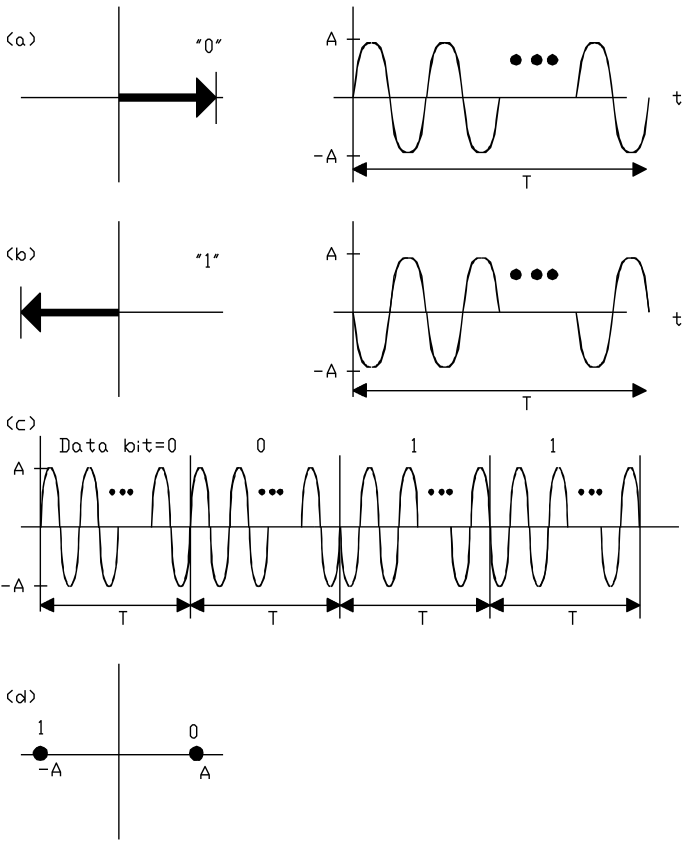
\includegraphics[width=0.55\linewidth]{figs/ch2_secMod_fig1.png}
    \caption{Example of \ac{iq} modulation \cite{Ha2010TheorySystems}}
    \label{fig:ch2_secMod_fig1}
\end{figure}

\par As such, the bits transmitted are represented as positions on an axis of a 2D-space, which is  shown in Figure \ref{fig:ch2_secMod_fig1} (d).

\par Although this figure is just for one of the data signals, \ac{i}, the fact that the quadrature signal \ac{q} is offset $90^{\circ}$ means that it would sit on a perpendicular axis creating a constellation of four symbols as shown in Figure \ref{fig:ch2_secMod_fig2}.

\begin{figure}[H]
    \vspace*{0cm}
    \centering
	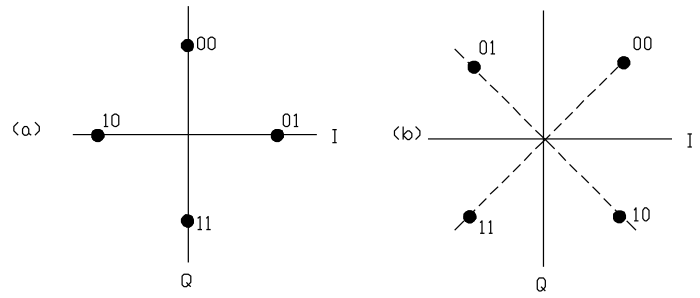
\includegraphics[width=0.5\linewidth]{figs/ch2_secMod_fig2.png}
    \caption{Example for two types of constellation for four symbols \cite{Ha2010TheorySystems}}
    \label{fig:ch2_secMod_fig2}
\end{figure}

\par In Figure \ref{fig:ch2_secMod_fig2}(a) we can observe the simpler case when constellation symbols sit on top of the axes of the graph. This is convenient as the coordinates present us directly with the amplitude for each symbol, but not mandatory. In Figure  \ref{fig:ch2_secMod_fig2}(b), we have the constellation skewed by $45^{\circ}$ and as such the symbols do not lie directly on top of the axes, and the amplitude of each symbol is not directly obtained.

\par More complex \ac{iq} modulation systems may have a multitude of constellations, usually with an amount of symbols that is a multiple of 2. This happens not only because we are modulating using the phase for each symbol but also the amplitude of the signals. As such, we have \ac{qam}.

\section{Phase Shift Arrays}
\label{section:ch2_psa}

\par \ac{psa} are considered a notable advancement in antenna technology. These have greatly influenced modern communications, radar, among several other applications. These are designed to very  carefully manipulate the phase of electromagnetic waves generated on individual elements of the array. This precise control of the phase enables \ac{psa} to use beamforming, beam steering, and adaptive signal processing on their operations to fulfill critical functions and applications.

\par The most relevant characteristic of \ac{psa} is the ability to shift phases. Traditionally, an antenna or array of antennas will receive or transmit a signal. This causes them to have a beam pattern that cannot change their form or direction unless they are moved. However, this does not hold on \ac{psa} that allow for an individual dynamic control of the phase of each antenna element relative to all the other elements. When a change is applied to the phase of these elements, the interaction between the electromagnetic waves also changes, resulting in different interference patterns that can be constructive or destructive in their influence. These can be controlled to achieve the desired characteristics of the beam. There are certain designs of \ac{psa} that can control the amplitude of the waves to shape the interference patterns of the array. There is also another advantage to arrays of antennas that comes in smaller side lobes due to the ability to control the shape of radiation being emitted.

\par The concept of multi-antenna array configurations has existed since the dawn of radio telecommunications, with several elements being synchronized in order to enhance both reception and transmission of radiation. In 1902, Nobel laureate Ferdinand Braun was already successful in transmitting directed wireless telegraph messages using inclined beam antennas \cite{NobelPrize.org2023FerdinandBiographical}.

\par Later advancements were more prominent during the mid-last century as a push towards improving \ac{par} was necessary due to their usefulness during WWI as they were capable of, for example, ground-controlled approach that allowed tracking airplanes and aid traffic controllers to guide pilots during bad visibility conditions.

\par Eventually the advantages of these radar arrays were applied to civilian telecommunications as well. As this happened, there was a shift from fixed antennas to electronically steerable ones. With these, wireless communication systems saw a facilitation in beamforming and beam steering techniques in order to increase efficiency of networks.

\par Nowadays, the evolution of \ac{psa} continues to advance, with the engineering and scientific communities making efforts to reduce both production costs and wasted energy, as well as expanding their range of applications. \ac{psa} have been used on 5G wireless networks, satellite communication systems, or vehicles, as examples.

\par For simplicity, we are going to consider that the distance between every element of the array is going to be constant, and for better performance, a distance of half of the wavelength of the carrier wave.

\subsection{Near Field vs Far Field}
\par The terms Near Field and Far Field serve as indications for the positioning of the \ac{rf} source relating to the \ac{psa}.

\par In Near Field circumstances, our \ac{rf}, from an isotropic antenna, source will be so close to our receiver that the wavefront propagating in front of the array will seem round, or not necessarily perpendicular to all elements of the \ac{psa}. In these situations, the waves arriving at the extremities of the array will be doing so later than they did at the center.

\par Far Field would then be a situation where the \ac{rf} source is positioned in front of the array, but so distant that the wavefront will seem parallel to the \ac{psa}, meaning that it will reach all elements with a delay that can be considered negligible.

\par The criteria adopted to distinguish between these two scenarios are usually described in (\ref{eq:ch2_farfield}). Here, D is the distance between the center of the first element and the last and $\lambda$ is the wavelength of the carrier wave.

\begin{equation}
    \label{eq:ch2_farfield}
    Far Field > 2\cdot\frac{D^{2}}{\lambda}
\end{equation}

\par This equation also allows us to determine that for arrays of small dimensions or for \ac{rf} sources of large wavelengths the distance at which we can consider that we are in Far Field territory is small. On the other hand, for larger arrays or for higher frequencies, the Far Field will happen much further from the \ac{psa}.

\subsection{Beamforming}
\par Beamforming is a technique that has been most useful for telecommunications, specifically for applications on \ac{psa}, as it enables the control of both shape and direction of radiation with precision. As such, performance and specific functionality for several applications is also increased.

\par We can distinguish between two major forms of this technique. There is analog beamforming that through phase shifters or attenuators allows for a less flexible approach. There is also digital beam forming, relying on \ac{dsp} technology to manipulate signals in the digital domain, resulting in more flexible and adaptable implementations, thus being more useful in a wider range of applications.

\subsubsection{Time-Domain Beamforming}
\par For this type of beamforming, the signal being transmitted or received by the array is time delayed or has its phase shifted from antenna to antenna as can be seen in Figure \ref{fig:ch_2_secArray_Array_Time_Delay}.

\begin{figure}[H]
    \vspace*{0cm}
    \centering
    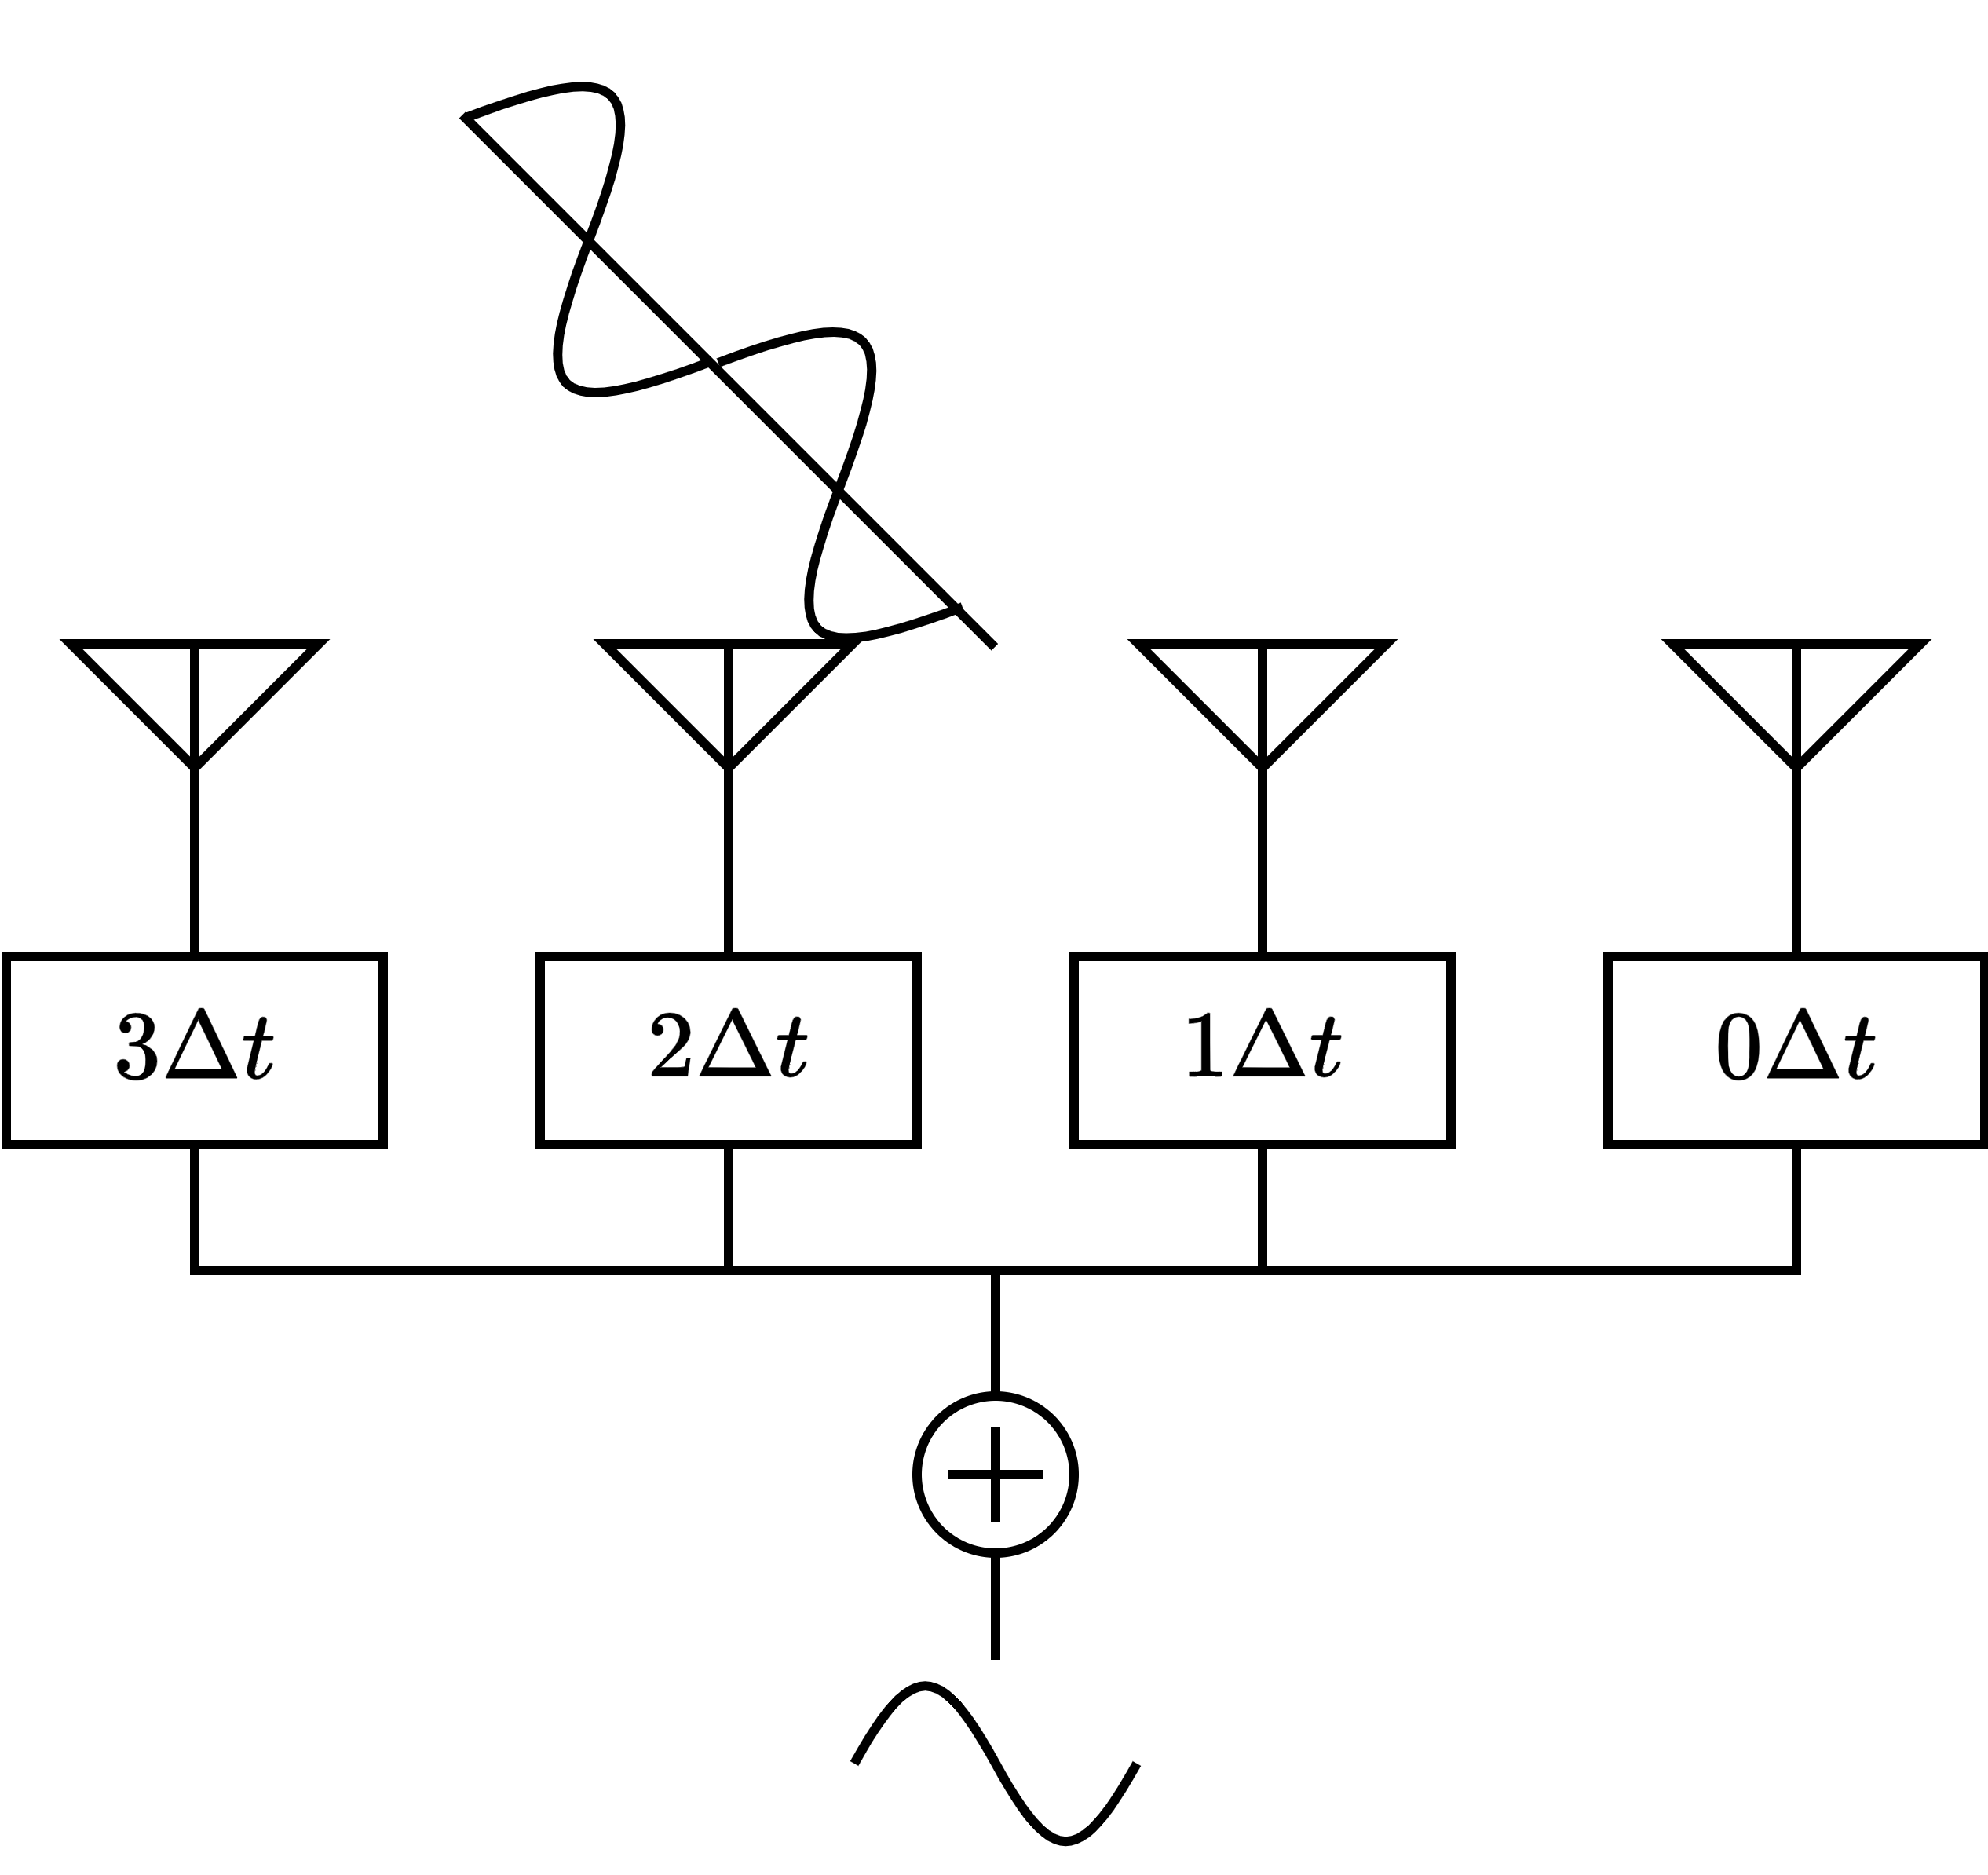
\includegraphics[width=0.5\linewidth]{figs/ch_2_secArray_Array_Time_Delay.png}
    \caption{Example for Time-Domain beamforming of 4 element array}
    \label{fig:ch_2_secArray_Array_Time_Delay}
\end{figure}

\par For far field applications this means that a wavefront of $45^{\circ}$ inclination will see time delays multiple of $\Delta$t applied at their path in the array, which are then summed together in order to have a more substantial signal at the output of the combining block.

\par The delay considered, $\Delta t$, can be calculated from (\ref{eq:ch2_timedelay}) \cite{Jang2018ABeamformer} where $\lambda$ is considered the wavelength of the carrier wave, $\Psi$ the angle of the beam and c is the speed of light.

\begin{equation}
    \label{eq:ch2_timedelay}
    \Delta t = \frac{\lambda}{2}\cdot\frac{\sin{\Psi}}{c}
\end{equation}

\par It is easily deduced from this equation that for applications where the wavefront is perpendicular to the array, when $\Psi$ is 0, there is no need for any delay, as the result of this equation is also zero, as one may expect. For all other situations where the wavefront and array are not perpendicular, this time delay is needed to achieve the best results possible on the array.

\subsubsection{Phase Shifting Beamforming}
\par This technique is very similar to the previous one, but we express the time delays as phase shifts. Considering that all the antennas in the array are at a distance, \textit{d}, of each other such that $d=\lambda/2$.

\begin{figure}[H]
    \vspace*{0cm}
    \centering
    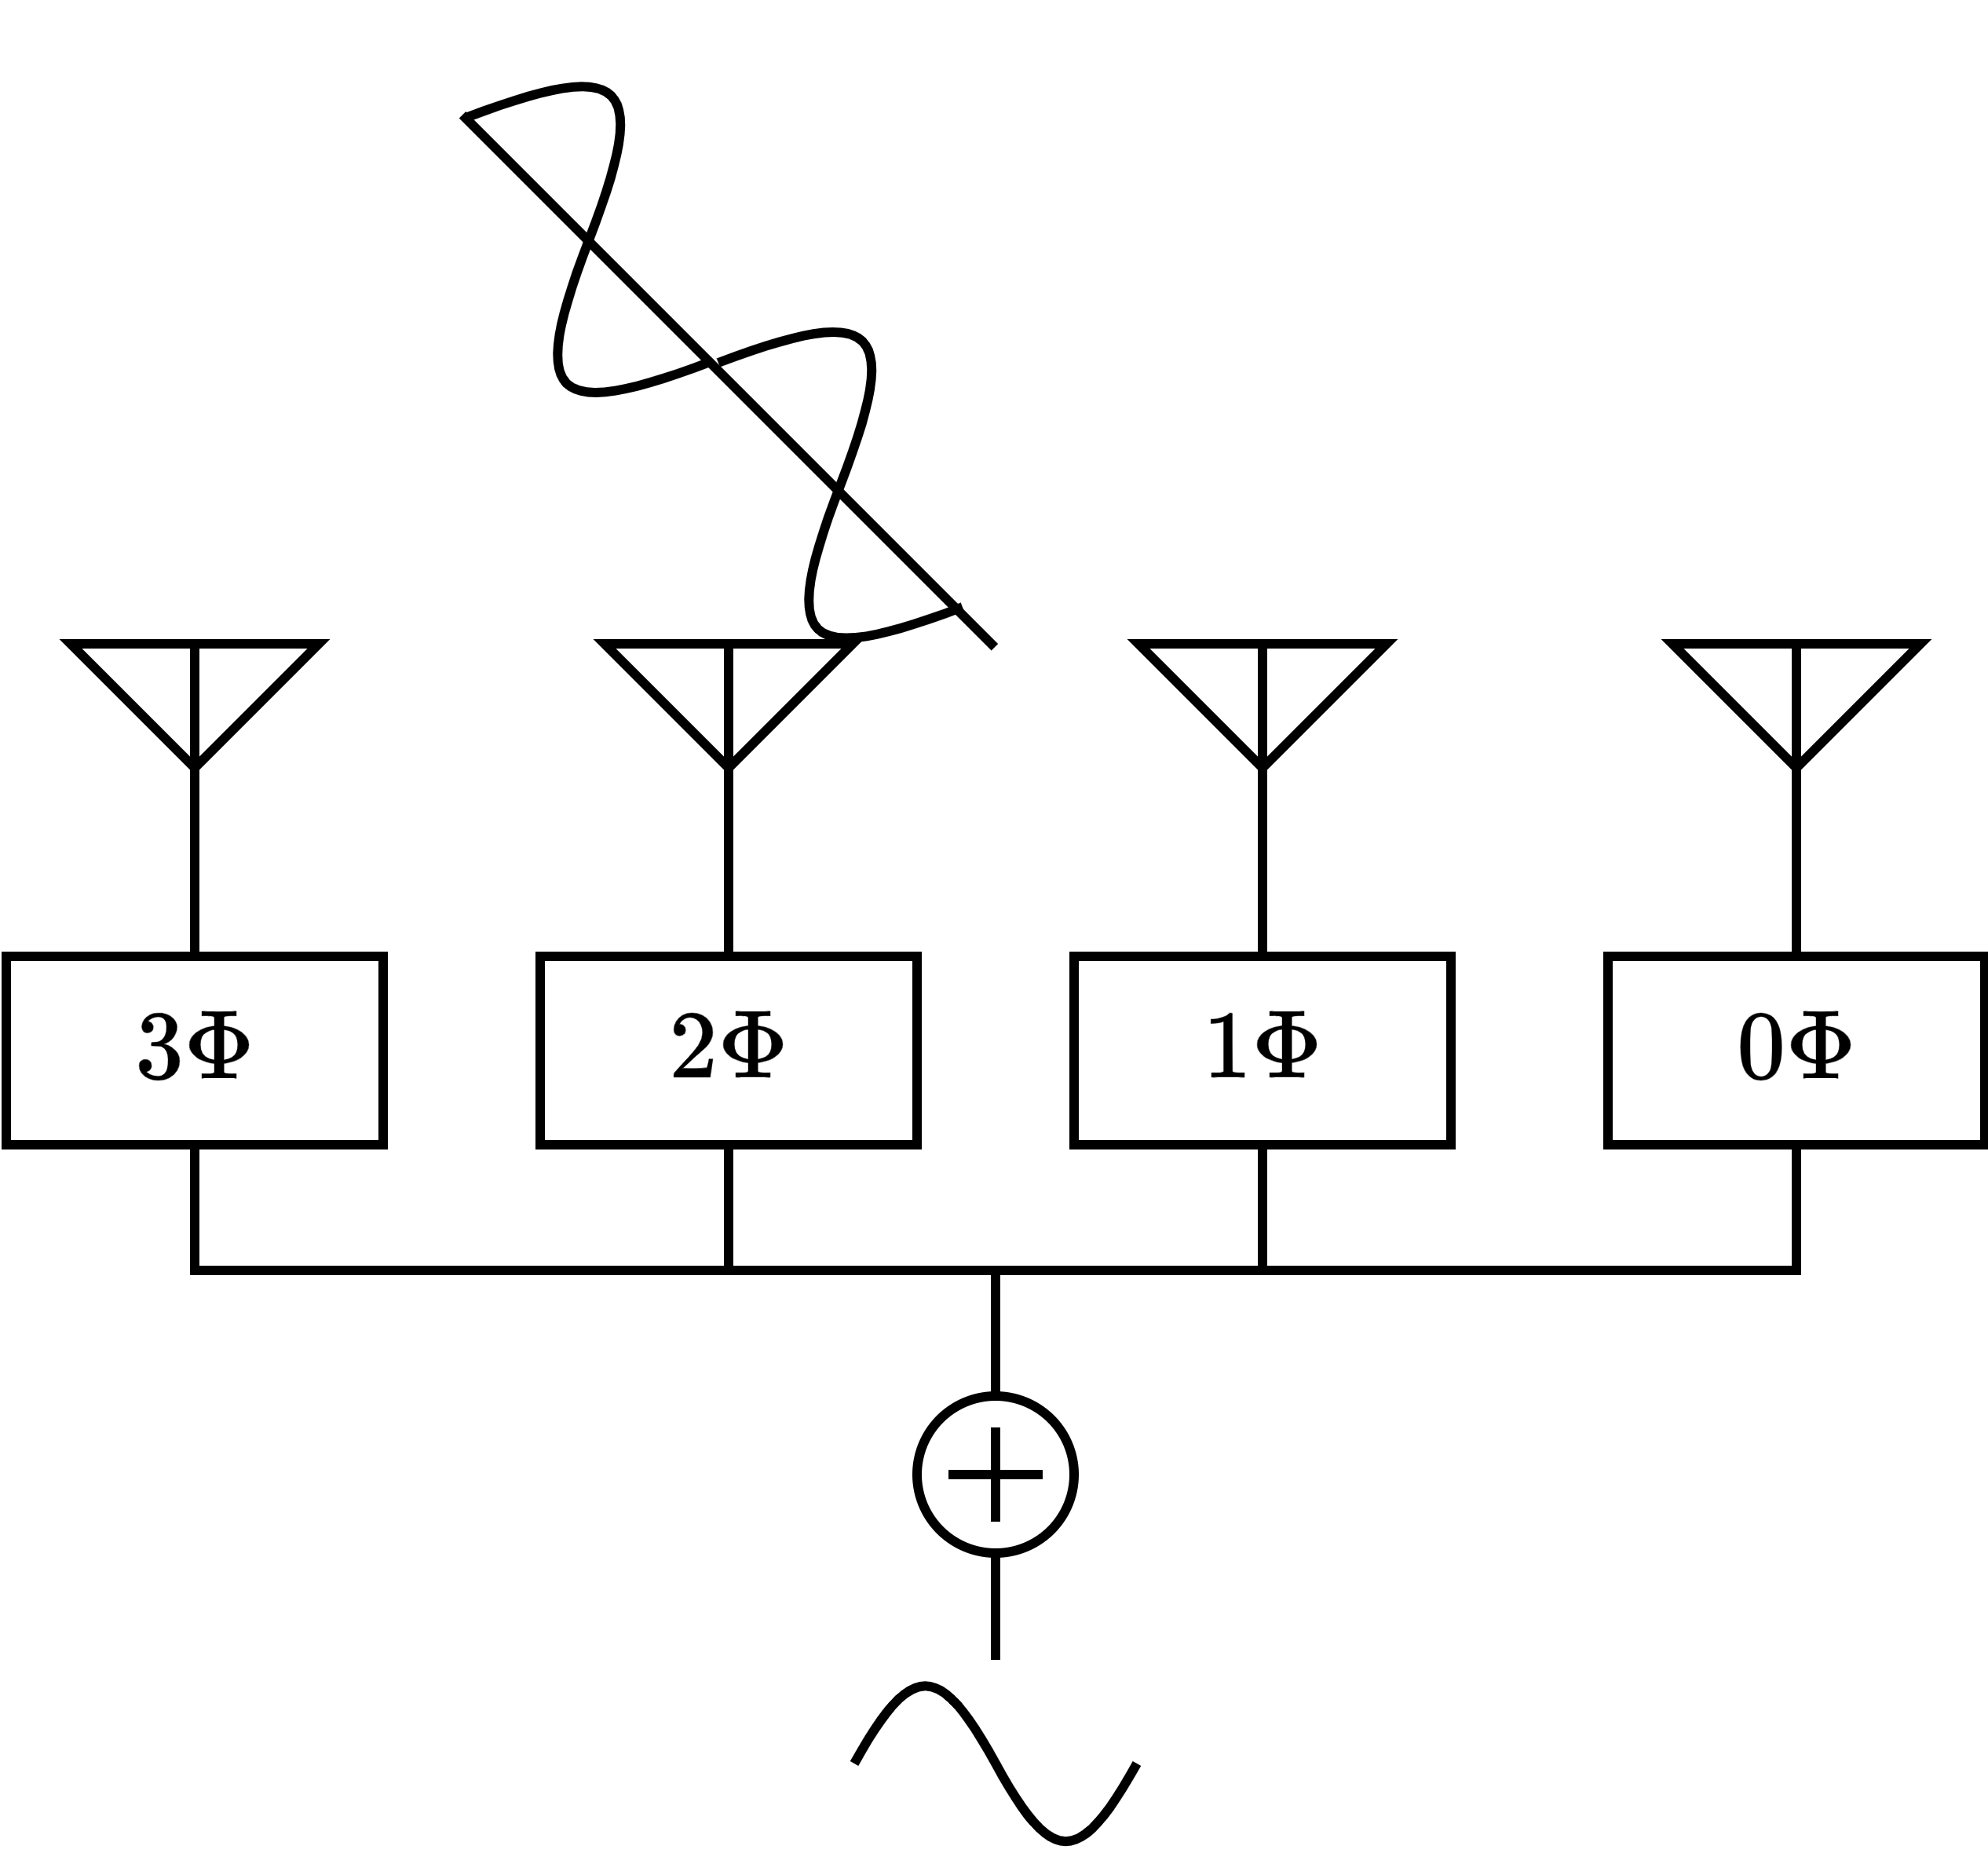
\includegraphics[width=0.5\linewidth]{figs/ch_2_secArray_Array_Phase_Shift.png}
    \caption{Example for phase shift beamforming of 4 element array}
    \label{fig:ch_2_secArray_Array_Phase_Shift}
\end{figure}

\par In this situation, $\theta$ is the inclination away from the perpendicular line of the array. Equation (\ref{eq:ch2_phaseshift}) shows how to calculate the phase shift for each element of the array.

\begin{equation}
    \label{eq:ch2_phaseshift}
    \Phi t = \pi\cdot\sin{\theta}\; rad
\end{equation}

\par This simplifies the approach to beamforming by increasing the gain of the captured signal or the transmission of information.

\subsubsection{Digital Beamforming}
\par For \ac{dbf}, the signal being received or transmitted has, at some point, to be converted from analog to digital or digital to analog accordingly. 

\par Figure \ref{fig:ch_2_secArray_DigitalBeamforming} shows an example of a receiver using this technique.

\begin{figure}[H]
    \vspace*{0cm}
    \centering
    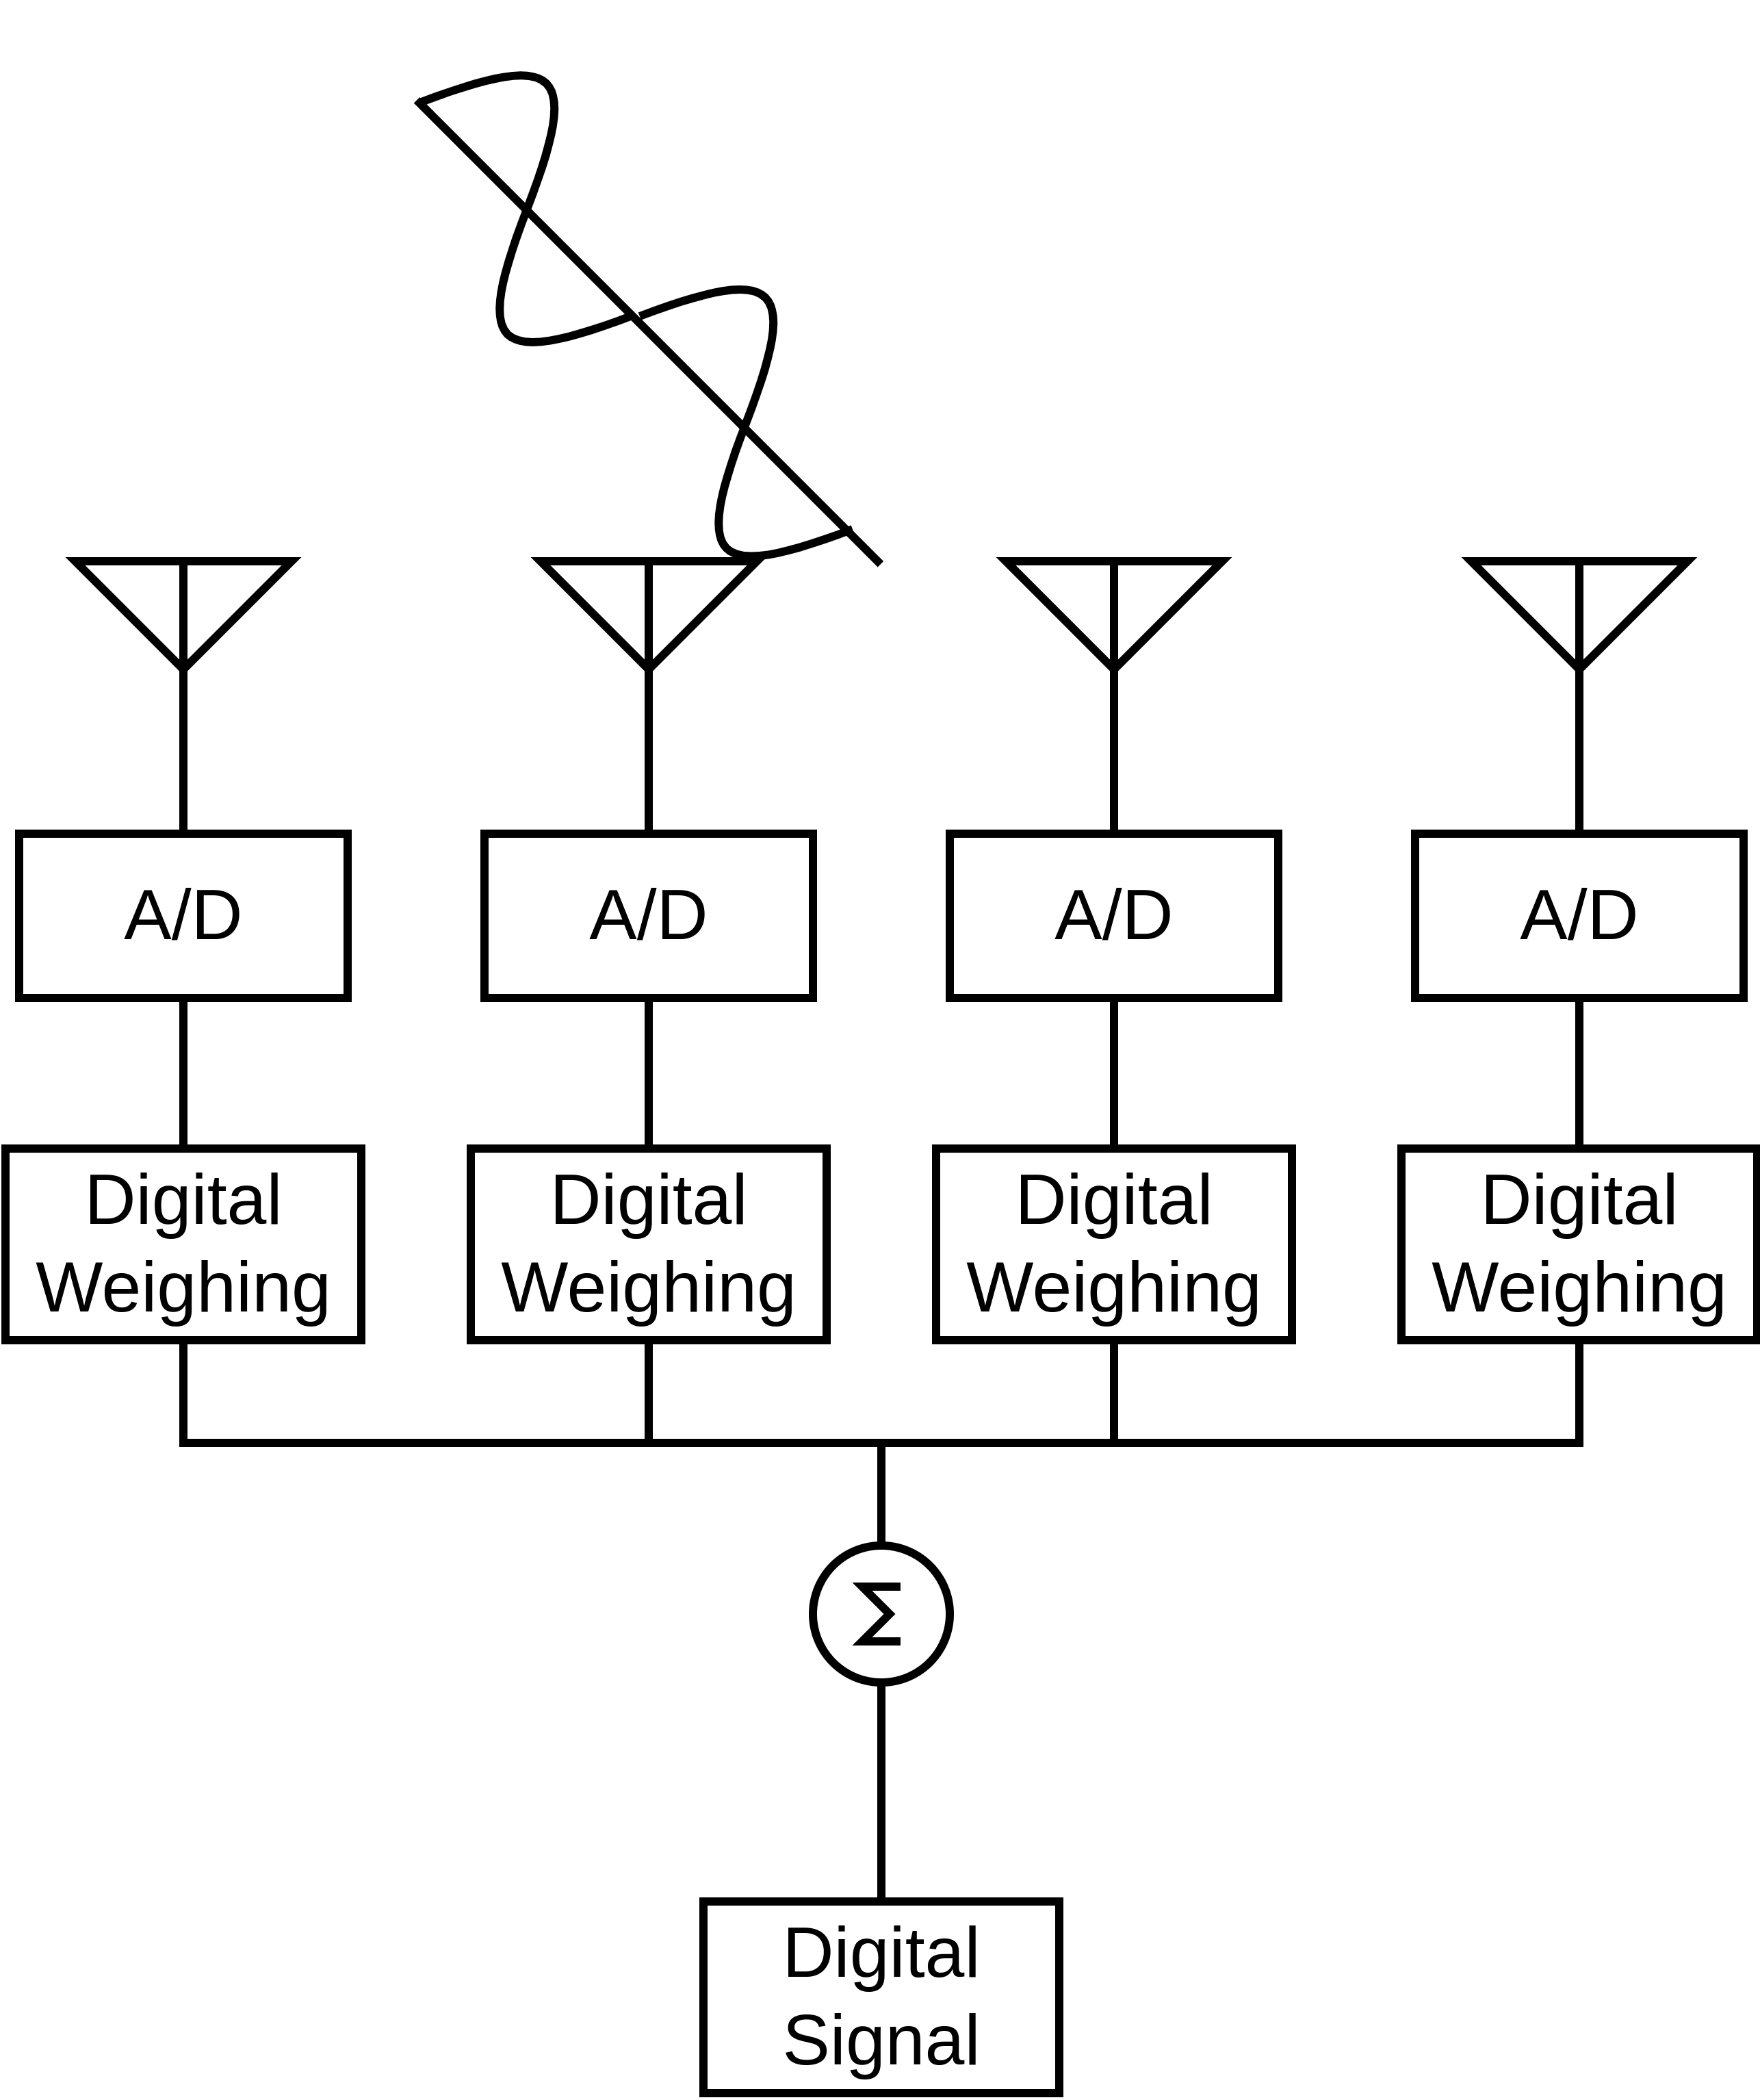
\includegraphics[width=0.5\linewidth]{figs/ch_2_secArray_DigitalBeamforming.png}
    \caption{Example for digital beamforming of 4 element array}
    \label{fig:ch_2_secArray_DigitalBeamforming}https://www.overleaf.com/project/6509e20fd9f6e5936b1c19ab
\end{figure}

\par The most obvious and logical benefit of using \ac{dbf} is that all data is readily available for digital processing, storage, and being worked on without loss to the information \cite{Kasemir2009WidebandBeamforming}. We also have the advantages of a better dynamic range, faster search frame times, and more precise control of both amplitude and phase to reduce sidelobe levels \cite{Skolnik2008RadarHandbook}.

\par One characteristic that cannot be overlooked in order to maintain good performance is the precision and speed of the converters. An optimal \ac{dbf} implementation would have ADCs or DACs with good resolution and fast maximum sampling rate. This would mean that very little to no information about the original data would be lost during the conversion process.

\par These systems, however, typically need a powerful \ac{dsp} or \ac{fpga} in order to process all the information set for transmission or that has been received and also to be able to keep up with the demands that result from the normal operation of the \ac{psa} such as being able to calculate all the variables needed to properly tune each element of the array to maintain proper functioning with the array calibrated to whatever angle needed. 

\par These problems are only exacerbated when high-speed information transfers are the target \cite{Lu2019ApplicationsSystem}, as the system will have to spend more computational resources for all tasks related to signal processing. The same holds true when the number of elements of the array increases, as it will be more taxing for the system to keep every element tuned for the particular situation.

\subsection{Beamwidth and Half-Power Beamwidth}
\par The \ac{ieee} defines beamwidth, or rather \ac{hpbw}, as "In a radiation-pattern cut containing the direction of the maximum of a lobe, the angle between the two directions in which the radiation intensity is one-half the maximum value" and defines the principal \ac{hpbw} as "For a pattern the major lobe of which has a half-power contour that is essentially elliptical, the half-power beamwidths in the two pattern cuts that respectively contain the major and minor axes of the ellipse"\cite{2014IEEEAntennas}.

\par These parameters are more specific to antennas than it is to \ac{psa} itself, but they are also important for the whole array of antennas. 

\par The previous definition regarding beamwidth is the separation in angle units for identical points in opposite sites of the maximum of the pattern. This can be expressed as an approximation in a horizontal coordinate system as shown in Equation (\ref{eq:ch2_beamwidth}) as $\Omega_{A}$.

\begin{equation}
    \label{eq:ch2_beamwidth}
    \Omega_{A} = \theta_{1}\cdot\theta_{2}\; (sr)
\end{equation}

\par In this equation, $\theta_{1}$ represents the azimuth and $ \theta_{2}$ is the elevation on the system used. The notion of depth is not considered, as we are looking only to evaluate the spherical area.

\par \ac{hpbw} is used to measure the angular distance between points of the main lobe of an antenna where the radiation pattern has lost half of its power related to the point of maximum power.

\par Equation (\ref{eq:ch2_hpbwangle}) gives the angle at which point \ac{hpbw} occurs. Equation (\ref{eq:ch2_hpbwsimple}) defines how to calculate \ac{hpbw}.

\begin{equation}
    \label{eq:ch2_hpbwangle}
    \theta  = \arcsin{ \frac{ 0.35 }{\pi }}\cdot\left(\frac{180}{pi}\right)\; (degrees)
\end{equation}

\begin{equation}
    \label{eq:ch2_hpbwsimple}
    HPBW  = 2\cdot\theta(degrees)
\end{equation}

\par Using Equation (\ref{eq:ch2_hpbw}) we can calculate the \ac{hpbw} of a linear and uniform array where N refers to the number of elements in a linear array, $\lambda$ is the wavelength of the carrier wave and $\theta$ is the angle of \ac{hpbw} and d is the distance between elements in this array. The angle $\theta$ refers to the beam angle.

\begin{equation}
    \label{eq:ch2_hpbw}
    \theta_{B}\approx\frac{0.886\lambda}{N\cdot d\cdot\cos{\theta}}
\end{equation}



\par There are also regions of the radiation-pattern that may see null power. Other regions may have less power being radiated through them. The last of these are known as the minor lobes. 

\par All of these characteristics can be observed in Fig. \ref{fig:ch_2_secArray_Beam}. This is a simple representation of a radiation pattern, however, these can be quite complex with several side lobes and multiple nulls.

\begin{figure}[H]
    \vspace*{0cm}
    \centering
    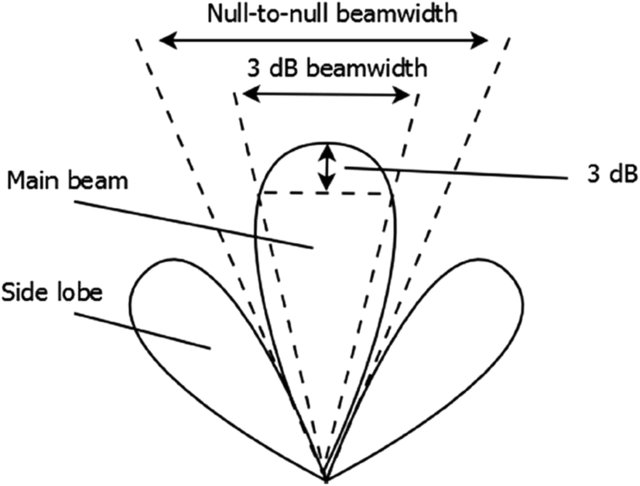
\includegraphics[width=0.5\linewidth]{figs/ch_2_secArray_Beam.jpg}
    \caption{Characteristics of radiation-pattern \cite{Bhattacharyya2020RadiationArrays}}
    \label{fig:ch_2_secArray_Beam}
\end{figure}

\subsection{Antenna Directivity}

\par Antenna directivity is a measurement of a characteristic of an antenna that is compared to an ideal isotropic antenna. This metric is also useful when there is need to evaluate the ability to focus the energy being radiated by the antenna.

\par Directivity is a dimentionless relationship of the antenna's maximum power $P_{MAX}$ and the average power that is radiated in all directions. 

\par For anisotropic antennas, when no direction is given, we consider the direction of maximum radiation intensity \cite{ConstantineA.Balanis2016AntennaDesign}. Equation (\ref{eq:ch2_maxdirectivity}) helps define this parameter, where $D_{0}$ is the maximum directivity, $U_{MAX}\;(W\cdot sr)$ is the maximum radiation intensity and $P_{RAD}\;(W)$ is the total radiated power of the antenna.

\begin{equation}
    \label{eq:ch2_maxdirectivity}
    D_{0}=\frac{4\cdot\pi\cdot U_{MAX}}{P_{RAD}}
\end{equation}

\par When an antenna has orthogonal polarization components, \citeauthor{ConstantineA.Balanis2016AntennaDesign} defines $D_{0}$ for a spherical coordinate systemn as shown in equation (\ref{eq:ch2_orthodirectivity}).

\begin{equation}
    \label{eq:ch2_orthodirectivity}
    D_{0}=D_{\theta}+D_{\phi}
\end{equation}

\par Here, the components for the partial directivies $D_{\theta}$ and $D_{\phi}$ are defined in (\ref{eq:ch2_orthodirectivitytheta}) and (\ref{eq:ch2_orthodirectivityphi}) respectively for each of the orthogonal field components.

\begin{align}
    D_{\theta} &= \frac{4\cdot\pi\cdot  U_{\theta}}{(P_{RAD})_{\theta}+(P_{RAD})_{\phi}}
    \label{eq:ch2_orthodirectivitytheta} \\
    D_{\phi} &= \frac{4\cdot\pi\cdot  U_{\phi}}{(P_{RAD})_{\theta}+(P_{RAD})_{\phi}}
    \label{eq:ch2_orthodirectivityphi}
\end{align}

\subsection{Antenna Gain}
This is a metric typically used to describe the gain of the antenna in a given direction. It evaluates the efficiency of the antenna with its directivity. It is described in Equation \ref{eq:ch2_antennagain}

\begin{equation}
    \label{eq:ch2_antennagain}
    G =  \frac{P_{RAD}}{P_{INPUT}}\cdot D_{0}
\end{equation}

\par Here, $P_{RAD}$ is the total amount of radiation power that the antenna is capable of outputting when a certain power, $P_{INPUT}$, is being supplied.

\subsection{Aperture}
\par Maximum effective aperture evaluates how well an antenna can receive radiation and the wavelength of the electromagnetic wave. The effective aperture for antenna, $A_{E}$, can be calculated using Equation (\ref{eq:ch2_antennaaperture}) \cite{Delos2020PhasedFactor}. Typically, this parameter is used on the direction of maximum radiation intensity \cite{ConstantineA.Balanis2016AntennaDesign}.

\begin{equation}
    \label{eq:ch2_antennaaperture}
    A_{E} = \frac{G\cdot \lambda^{2}}{4\cdot\pi}
\end{equation}


\subsection{Array Factor}
\par \ac{af} is a metric used to express the combined radiation pattern of the eletctromagnetic contributions of all individual elements in a matrix. By helping to understand how all individual radiating elements in the array interact with each other and, as a whole, generate the radiation pattern of the array, \ac{af} is one useful tool in the process of optimizing the performance of the array for the specific application that it is designed to accomplish.

\par This function depends on the position of each antenna element of the matrix, the phase and amplitude of their respective electromagnetic fields relative to other elements in the matrix and certain characteristics specific to the antennas themselves.

\par This means that each array, due to all the possibilities within these parameters, has a specific \ac{af} of its own. As there is no dependency of the \ac{af} with the directional characteristics of the antennas \cite{ConstantineA.Balanis2016AntennaDesign}, we can simplify the calculation process by considering each antenna in the array as isotropic. In this way, \citeauthor{ConstantineA.Balanis2016AntennaDesign} defines the total field of an array as in Equation (\ref{ch2_totalfieldarray}).

\begin{equation}
    \label{ch2_totalfieldarray}
    E_{TOTAL} = E_{element}\cdot AF(\theta)
\end{equation}

\par The value for \ac{af} for the center of the array is given by Equation (\ref{ch2_arrayfactor})\cite{Delos2020PhasedFactor}.

\begin{equation}
    \label{ch2_arrayfactor}
    AF(\theta) = \frac{\sin(\frac{N}{2}\cdot\Psi)}{\sin(\frac{N}{2}\cdot\Psi)}
\end{equation}

\par Here, $\Psi$ represents the phase difference from the previous element of the array, and N is the total number of elements in the array.

\subsection{Grating Lobes}
\par Grating lobes are secondary radiation lobes that are observed when, in antenna arrays, the distance between the radiating elements of the array is less than half of the desired wavelength of the array. They are taken into consideration in those conditions as they appear due to the periodicity of antenna arrays. These can be harmful to the overall operation of the array.

\par These can cause interference in communication systems with nearby sections of the electromagnetic spectrum and disrupt the performance of the array, leading to a loss in directivity or the ability of the antenna array to focus its beam.

\par Figure \ref{fig:ch2_secArray_GratingLobes.png} shows how a different spacing on 32 elements of an array, despite not necessarily decreasing the intensity of the main lobe, significantly changes the format of the radiation-pattern and demonstrates the existence of a now new lobe when the phase of the array is shifted.

\begin{figure}[H]
    \vspace*{0cm}
    \centering
    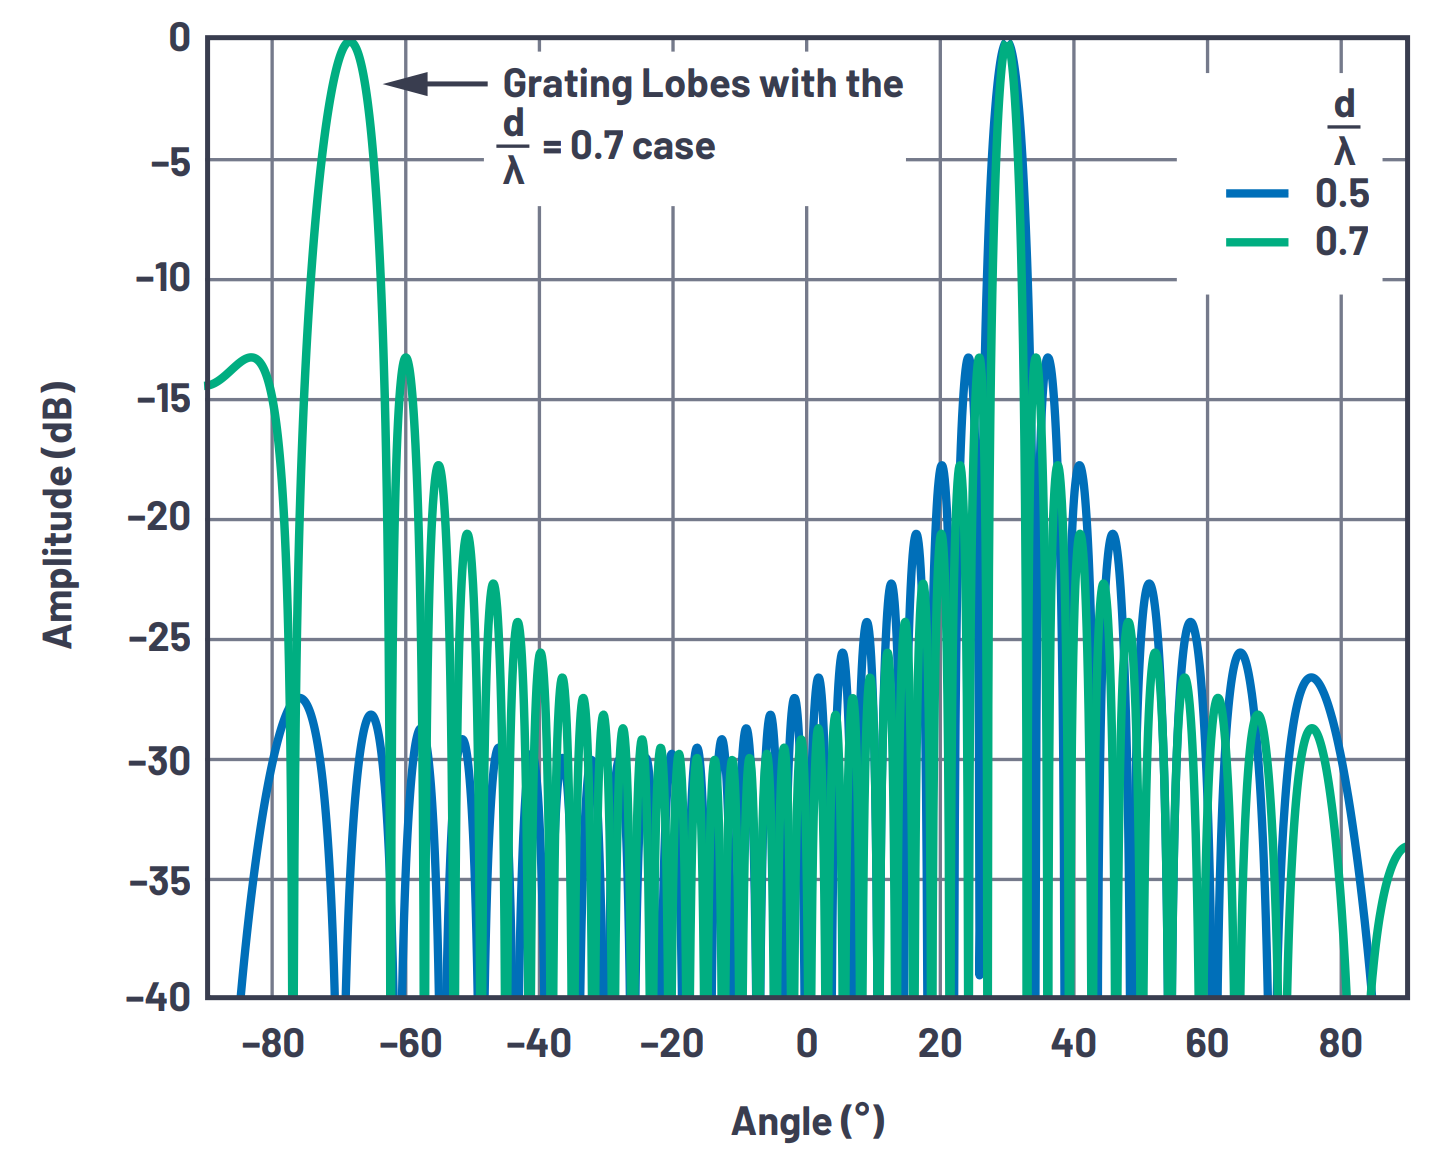
\includegraphics[width=0.5\linewidth]{figs/ch2_secArray_GratingLobes.png}
    \caption{Grating Lobes for 32 element array \cite{Delos2020PhasedTapering}}
    \label{fig:ch2_secArray_GratingLobes.png}
\end{figure}


\par According to \citeauthor{Delos2020PhasedTapering}, we can obtain at what beam angle we obtain grating lobes if we consider the solutions of (\ref{ch2_gratinglobes}).

\begin{equation}
    \label{ch2_gratinglobes}
    \theta = \arcsin{\left(\frac{\lambda}{d}\cdot \left( m + \frac{d\cdot\sin{\theta}}{\lambda} \right)\right)}
\end{equation}

\par Here, \textit{d} is the distance between elements, $\lambda$ the wavelength of the carrier and \textit{m} is all possible spatial images for the appearance of a periodic replica. The value of \textit{m} can be any possibility within the sequence $m = \pm1, \pm2, etc$.

\par When the solution of the equation is a single real number, we are able to avoid its presence, which means that for $m\geq1$ Equation (\ref{ch2_gratinglobescondition}) must be true.

\begin{equation}
    \label{ch2_gratinglobescondition}
    1 < \left|\frac{\lambda}{d}\cdot \left( m + \frac{d\cdot\sin{\theta}}{\lambda} \right)\right|
\end{equation}

\par When this relation is not met for $m > 0$, then $\arcsin$ returns a real number that results in a grating lobe. If the solution is otherwise an imaginary number, then it can be ignored. 

\subsection{Spacing between radiating elements}
\par We know that when distance for ajdacent antennas in the array is $\lambda/2$ there is not interference between the radiation of neighboring elements. However, for distances above $\lambda/2$ there is a risk that grating lobes appear causing problems on the array's behavior due to spacial aliasing, and we can use the Nyquist theorem in this context \cite{Delos2020PhasedSquint}. 

\par This parameter should be considered when designing the array, as it may come as a trade-off between the size of the array, the size of the scanning angle, operating frequency, and the occurrence of these undesirable phenomena.

\subsection{Mutual Coupling}
\par In \ac{psa}, each radiating element can be influenced by and influence its neighbouring elements. This can introduce challenges that limit the performance of the system. Each element's performance changes depending on how closely or sparsely they are from one another in the array, for example. But there can be other factors that can cause mutual coupling, other than the simple geometric position of the radiating elements of the array. Operating frequency, due to the size of the wavelengths being considered, the steering of the radiation-pattern and the presence of conducting materials in the \ac{psa}.

\par Also, not all elements will suffer from mutual coupling to the same extent. One can see that in a square array of $N\times N$ elements, the ones on the corners will have fewer surrounding neighbors, followed by all the other ones on the edges, and as we reach closer to the center of the array, this effect might keep changing. 

\subsection{Beam Angle Resolution}
\par As seen previously, these devices can be controlled by timed delay or phase shift. These do not produce continuous intervals of numbers. Most have a maximum resolution that they can work with. They exist in discrete domains where both time and phase intervals have steps. And this problem is insensitive to whether the system is being controlled via an analog signal or digitally.

\par For analog systems, this is a very straightforward process. A small amount of voltage or current will increase the time delay or phase shift by a certain amount. But for digitally controlled systems we have to wonder how many bits do we need to change the time delay or phase shift.

\par For cases where a phase shifter is used, the resolution of the \ac{psa} will differ from the resolution of the phase shift used, as expected. Equation (\ref{ch2_angleLSB}) establishes the relationship between the number of bits, B, of the phase shifter and its angle resolution.

\begin{equation}
    \label{ch2_angleLSB}
    \Phi_{LSB} = \frac{\pi}{2^{B}}
\end{equation}

\par If we consider Equation (\ref{ch2_gratinglobes}) seen previously, for a linear array of \textit{N} elements spaced by half a wavelength, we obtain an angle resolution $\theta_{R}$ in relation to the angle resolution in bits, $\Phi_{LSB}$, as shown in Equation (\ref{ch2_beamResLSB}).

\begin{equation}
    \label{ch2_beamResLSB}
    \theta_{R}\approx\arcsin{\frac{\Phi_{LSB}}{N\cdot\pi}} \text{\cite{Delos2020PhasedDevicesc}}
\end{equation}

\par Figure \ref{fig:ch_2_secArray_PhaseResElements.png} details how Equation (\ref{ch2_beamResLSB}) expresses the resolution of the beam angle with the total number of elements in a linear array spaced by half of a wavelength according for different phase shifters with different $\Phi_{LSB}$. In this Figure, it can be seen that for phase shifters with only two bits, as blue, the resolution is worse than for the case when the phase shifter has 4 bits, seen in purple, for example.
\begin{figure}[H]
    \vspace*{0cm}
    \centering
    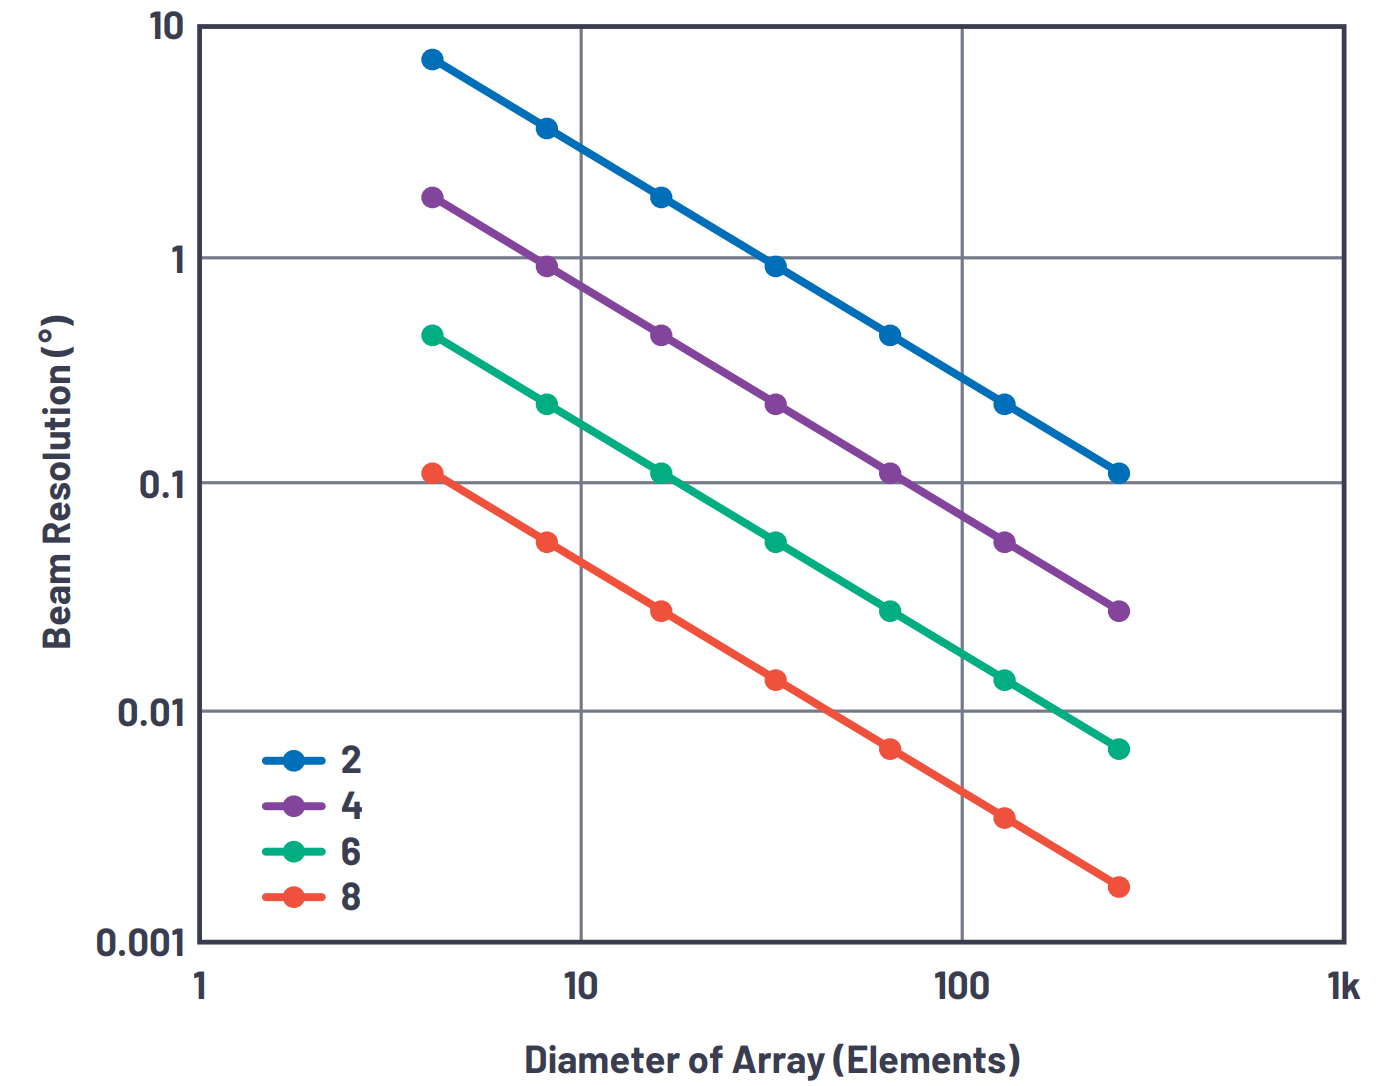
\includegraphics[width=0.5\linewidth]{figs/ch_2_secArray_PhaseResElements.png}
    \caption{Beam angle resolution relation with the array number of elements for various phase shift resolution\cite{Delos2020PhasedDevicesc}}
    \label{fig:ch_2_secArray_PhaseResElements.png}
\end{figure}

\par This helps to visualize how the bit resolution of the phase shifter can influence the total amount of beam angle resolution of the array. It also demonstrates the importance of choosing the right phase shifter with and appropriate $\Phi_{LSB}$ for what is expected of the \ac{psa} that is being designed. As expected, the smaller $\Phi_{LSB}$ is then the better is the beam resolution of the array. This is particularly important for systems that have a small number of elements, or we may see that beam resolution may negatively affected the whole operation of the system, providing poor beamforming capabilities.

\par However, even a phase shifter with a $\Phi_{LSB} = 90^{\circ}$, which means two bits total, can achieve a small beam resolution for arrays with large numbers of elements.

\subsection{Quantization of Sidelobes}
\par Phase shifters with larger $\Phi_{LSB}$ resolutions tend to be a hindrance to system gain.
\par \citeauthor{Skolnik2008RadarHandbook} explains that the relation between the total number of bits, \textit{B}, of a phase shifter and the loss in gain of the system is defined in Equation (\ref{ch2_GainLossLSB}).

\begin{equation}
    \label{ch2_GainLossLSB}
    \Delta G = \frac{\pi^{2}}{2^{2\cdot B}\cdot 3}
\end{equation}

\par The energy lost due to this effect is then divided along the side lobes of the system. It is easy to deduce that for systems where the phase shifter has a larger $\Phi_{LSB}$ resolution, the total loss in gain will be larger than if the \ac{psa} had a phase shifter with a small $\Phi_{LSB}$.

\par Figure \ref{fig:ch_2_secArray_QSLL.png} shows a visual representation of how the \ac{qsll}, in $\:\si{dB}$, relates to the number of bits of the phase shifter. 

\begin{figure}[H]
    \vspace*{0cm}
    \centering
    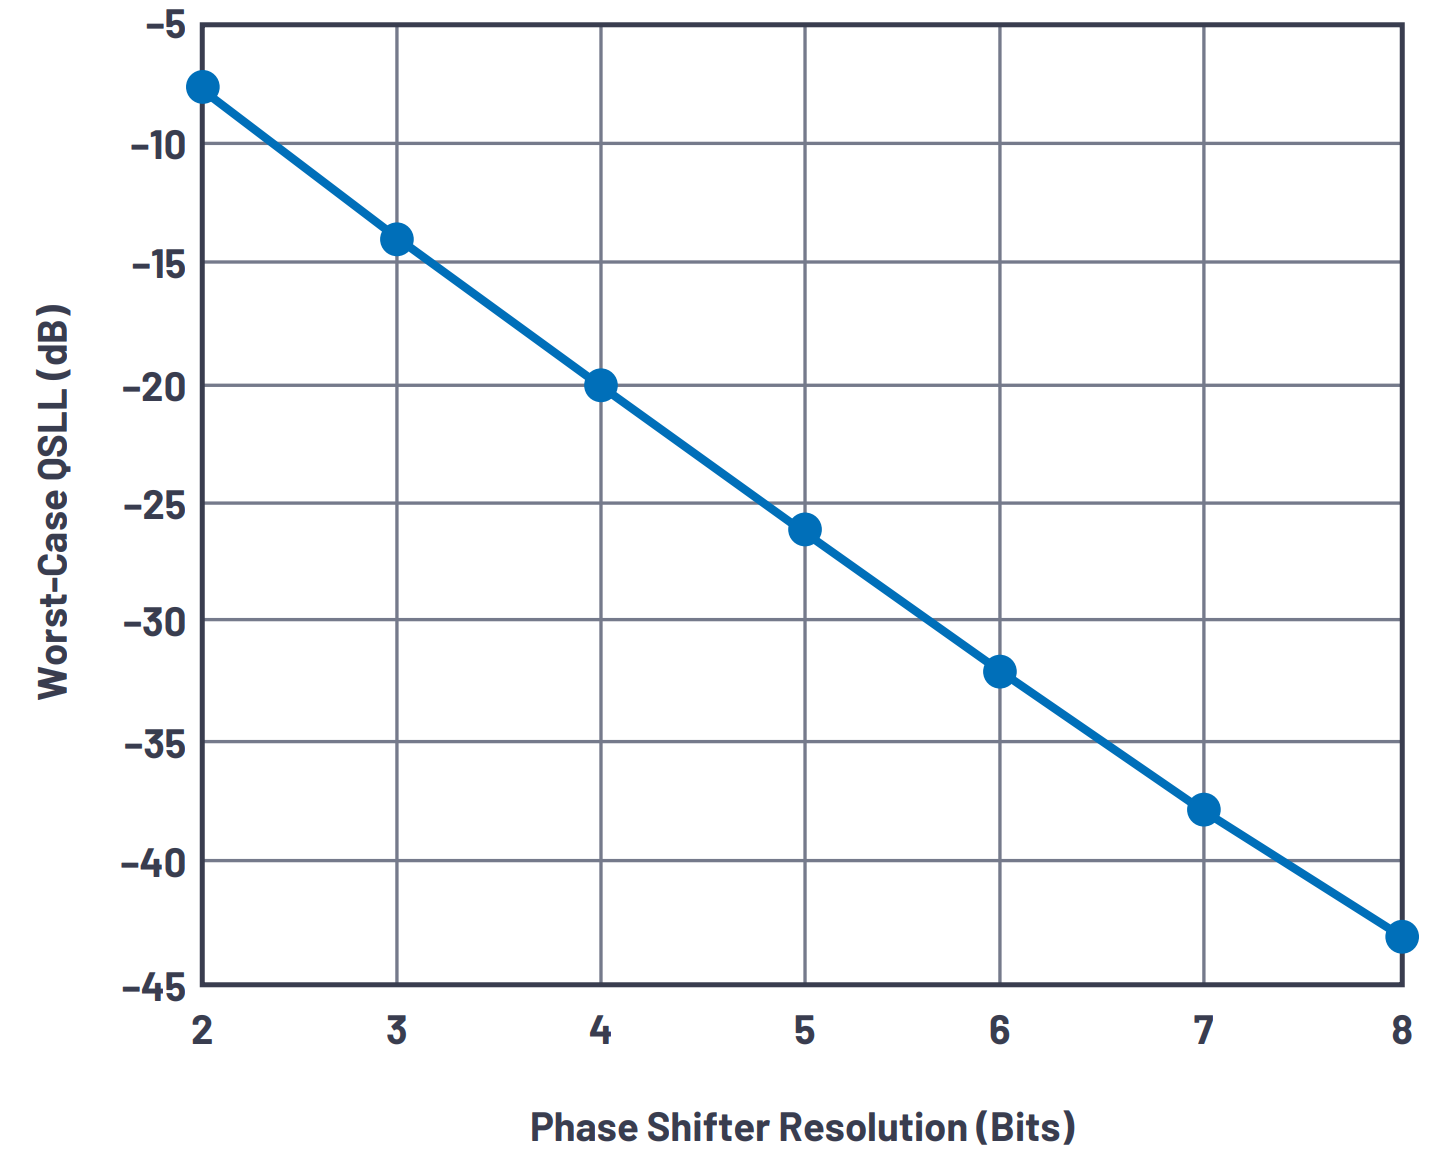
\includegraphics[width=0.5\linewidth]{figs/ch_2_secArray_QSLL.png}
    \caption{Quantization sidelobe levels relation with phase shifter resolution\cite{Delos2020PhasedDevicesc}}
    \label{fig:ch_2_secArray_QSLL.png}
\end{figure}

\subsection{Application of Phase Shift Arrays Nowadays}
\par These systems are extremely attractive in the realm of radar systems. From being used in armed forces all over the world to weather forecasting, air traffic control, and space exploration, they can be used due to their ability in manipulating the shape, angle, and directivity of their radiation-patterns, how easy it is to implement adaptive interference cancelation algorithms due to the number of antennas used, and good performance at tracking and distinguish signals.

\par They are a foundational equipment in telecommunication systems, due to their ability to beamform and allowing for beamsteering of the radiation pattern.

\par With the advent of 5G technology and the massive \ac{mimo} systems that come with, \ac{psa} have a pivotal role in the delivery of high-speed and low-latency communications that these modern applications require. The fact that many beams can be controlled on a one-to-one level is one big selling point for this field. 

\par \ac{psa} have also been used in the medical field, their implementation greatly benefiting the advances in medical imaging such as ultrasound and magnetic resonance imaging examination techniques. The enhanced resolution and overall quality of the images that are obtained, along with the ability to direct very precisely the radiation-patterns allows for more accurate diagnoses without the need for more invasive methods of the past, such as exploratory surgery.

\par Their use has also been helping physics and astronomers alike in the exploration of the universe because of their capabilities regarding beam steering that allows the study of specific regions or celestial objects.

\subsection{Benefits and Disadvantages of \ac{psa}}
\par In this section, the main identified advantages and disadvantages are outlined in the following paragraphs. 

\subsubsection{Advantages}
\par Easily the very first benefit that comes to mind for \ac{psa} is the exceptional and reliable ability to steer electromagnetic beams with very good precision. As such, all applications that benefit from beamstearing like tracking, reduced interference, and fine-tuned signal reception, can only be empowered by their use.

\par The enhanced efficiency of \ac{psa} is also to be noted here, as they can precisely concentrate energy where it is needed and minimize signal loss and interference that can result in higher data transfer rates and extended ranges.

\par As seen previously, \ac{psa} can be highly versatile with their use in various scientific fields, each with different operating frequencies and requirements.

\par The fact that they can be controlled electronically, instead of being fixed or relying on mechanical motors, allows swift adjustments to the direction of their beams and also their shape to better respond to the need of their application.

\subsubsection{Disadvantages}
\par High performance \ac{psa} can be costly. The development, deployment and maintenance of these systems, with specialized materials, components, and manufacturing processes, can contribute to an elevated cost that limits its accessibility for smaller-scale applications, although there have been efforts to integrate them as \ac{mmic}.

\par Another point of concern for \ac{psa} is their complexity. Both in design and operation, these are very complex pieces of technology that require an understanding of electromagnetic fields, some signal processing both for digital and analogue scenarios, and knowledge in control systems. This poses a challenge in terms of calibration and troubleshooting that requires skilled engineers and technicians to maintain proper operation.

\par Unfortunatly, \ac{psa} may require a substantial amount of electrical resources to remain operational. This restricts their usage in battery-powered devices or low-power applications.

\par Due to the large number of electronic components in a \ac{psa}, they can be susceptible to electromagnetic interference from external sources, which may hinder their deployment for certain applications where this factor could be a concern.

\section{\acl{mimo} Systems}
\par \ac{mimo} technology has been a cutting-edge development in wireless communications with a lot of focus on investigation and improvement over the last years \cite{Spencer2004AnDownlink}. With advancements in antenna arrays for both transmitter and receiver, helping to enhance the transmission of data over distance, allowing for bigger throughput and the system's performance \cite{Spencer2004AnDownlink}\cite{Alexandropoulos2022Full-DuplexDirections}\cite{Zhang2006FutureNetworks}.

\par \ac{mimo} technology emerged as a solution to the challenges wireless communication systems have been facing\cite{Spencer2004AnDownlink}. Typical wireless systems as we know them have faced problems with radio frequency spectrum limitations, with every frequency band being costly, multipath distortion that can be due to a variety of reasons, and interference \cite{Spencer2004AnDownlink}\cite{Lawton2008IsCommunications}. With data consumption continuously growing exponentially, and with no expectation for a decline in the near future due to the proliferation of smart devices, more streaming platforms that can range from normal media formats to cloud video gaming, \ac{iot} devices and applications, there has been an increased demand for higher data rates, with little to no dropped information, enhancing the networking capacity in order to provide a consistent quality service to all clients \cite{Spencer2004AnDownlink}.

\par \ac{mimo} technology then came as a technology that could address these constraints and overcome them. With the aid of sophisticated algorithms and antenna arrays, \ac{mimo} systems can simultaneously transmit and receive various data signals over the same radio channel \cite{Alexandropoulos2022Full-DuplexDirections}\cite{Zhang2006FutureNetworks}. This type of multiplexing is done by sending data over multiple paths, taking advantage of what conventional radio systems consider interference and fading \cite{Spencer2004AnDownlink}\cite{Alexandropoulos2022Full-DuplexDirections}. This effectively provides a significant boost to the system capacity and efficiency without the need for additional bandwidth or increase in transmission power needed for wireless communication \cite{Lawton2008IsCommunications}.

\par The flexibility and adaptability of these systems that, operating on the physical layer, can seamlessly integrate with several types of wireless transmission protocols, including the widely available and used Wi-Fi IEEE 802.11 standards \cite{Spencer2004AnDownlink}\cite{Lawton2008IsCommunications}.

\par Although \ac{mimo} technology has been developed to enhance wireless communications, it is not perfect: Energy consumption, financial cost, and competition from other parallel communication technologies may become hindrances in \ac{mimo} future development \cite{Rusek2013ScalingArrays}. However, the \ac{mimo} technology has been allowed a solid foothold with its integration into emerging broadband standards \cite{Zhang2006FutureNetworks}. This becomes more evident as major companies invest on the development of this technology with \ac{mimo}-based products.

\par There have been plans for the future development of large \ac{mimo} systems with a greater amount of antenna elements have been proposed than in today's setups, with the aim of being more efficient \cite{Zhang2006FutureNetworks}. Also, it is important to consider that the robustness of these systems also has room to improve. As systems grow in both scale and requirements, new implications in \ac{dsp}, programming, and network design are revealed \cite{Zhang2006FutureNetworks}. 

\subsection{Principles and Operations}
\par \ac{mimo} leverage the spatial dimension to improve the performance of the system. 

\subsubsection{Space-Time Modulation and Coding}
\par Unlike \ac{siso} systems, \ac{mimo} technology relationship between input and output cannot be described as if it were a scalar, rather they are described as a vector, for example $y=Hx+n$. The extension of space, by using several antenna elements, and time, with different symbol times, is commonly known as space-time coding \cite{Goldsmith2005WirelessCommunications}.

\par This technique allows for an easier way of understanding and implementing an algorithm where, with $M_{T}$ the number of antenna elements transmitting, $M_{R}$ the total number of antenna elements at the receiver and T the symbol times, we can express the input matrix as $X=[x_{1},...,x_{T}]$ for the input channel $M_{T}\times T$ and the channel output matrix for $M_{R}\times T$ expressed as $Y=[y_{1},...,y_{T}]$. We can also now add the noise that is captured by the receiver as $N=[n_{1},...n_{T}]$. The model that we arrive at can be described as shown in Equation (\ref{ch2_MatrixMIMO}) according to \citeauthor{Goldsmith2005WirelessCommunications}.

\begin{equation}
    \label{ch2_MatrixMIMO}
    Y=HX+N
\end{equation}

\subsubsection{Spatial Multiplexing}
\par One of the techniques used by multi-antenna arrays in \ac{mimo} technologies for smaller frequency bands consists of spatial multiplexing systems. This requires that the receiver end be able to demultiplex the transmitted information.

\par In a system described by the model suggested in Equation (\ref{ch2_MatrixMIMO}), the overall channel capacity, $C_{SM}$ is described by Equation (\ref{ch2_ChannelCapacity}).

\begin{equation}
    \label{ch2_ChannelCapacity}
    C_{SM} = \sum_{i=1}^{r} \log_2\left( 1+ \frac{\rho}{M_{T}}\cdot\lambda_{i}\right)
\end{equation}

\par Here, $\rho$ represents the signal-to-noise ratio, $\lambda_{i}$ is the i-th eigenvalue of the matrix $HH^{H}$ and r is the rank of this matrix\cite{Kalachikov2018PerformanceModels}.

\par In order for a receiver to distinguish one data stream from the interference of the other $M_{T}-1$ that are being transmitted, algorithms such as \ac{mmse} and \ac{zf} can be used.

\par For system using \ac{zf}, we can use the \ac{zf} equalizer $W_{ZF}$ shown in Equation (\ref{ch2_zfequal}) on the received data Y, in this case a vector, to retrieve the vector $x_{ZF}$ we are interested in shown in Equation (\ref{ch2_zfequal}) \cite{Mehana2012DiversityReceivers}. 

\begin{equation}
    \label{ch2_zfequal}
    W_{ZF} = (H^{H}H)^{-1}H^{H}
\end{equation}

\begin{equation}
    \label{ch2_zfequal}
    x_{ZF} = W_{ZF}y
\end{equation}

\par This technique can, however, lead to noise amplification problems. Therefore, this requires a \ac{mmse} equalizer to reduce this effect. Note that this also involves a more complex implementation. The output of this detector will then be as described by Equation (\ref{ch2_mmseequal}) where $\sigma$ is the known standard deviation of the noise present in the receiver\cite{Kalachikov2018PerformanceModels}.

\begin{equation}
    \label{ch2_mmseequal}
    x_{ZF} = (H^{T}H+\sigma^{2}I)^{-1}H^{T}y
\end{equation}

\subsubsection{Spatial Diversity}
\par Spatial diversity consists of employing several transmitters and receivers to provide some level of fading compensation. This also helps prevent situations where the signal is blocked due to some accidental obstacle in its way\cite{Navidpour2007BERDiversity}. 

\par This technique maintains high transmission rates when the number of antenna elements in the receiver is equal to the number of the transmitter. It is undesirable for number of elements of the receiver is larger than the number in the transmitter \cite{Bharati2020RealizationGains}.

\subsubsection{Channels}
\par In the model presented for \ac{mimo} systems, the matrix $H$ is used to represent the channel between the transmitter and the receiver. Characterizes the scattering of the propagation environment between multiple antennas at both ends of the channels. This matrix contains the relationships between the transmitter's and the receiver's antenna elements.

\par The channels characteristics have a profound impact on how signals are received and what decoding strategies must be used to establish proper communication, for example, based on the speed at which signals fade.

\subsubsection{\acl{snr} and \acl{sinr}}
\par Systems like that use \ac{mimo} technology suffer from what is known as \ac{sinr}. This metric establishes a relationship that also includes the effect of each channel being transmitted on the other channels present, unlike \ac{snr} that only takes into account the effects of noise present on the channel of interest.

\par If we consider $P_{R}$ the power of the channel's signal that is received, $N_{0}$ the noise power spectral 
density, $B$ the bandwidth of the channel and $P_{I}$ the power caused by interference of all the other channels, then Equation (\ref{ch2_sinr}) will define the total \ac{sinr} present.

\begin{equation}
    \label{ch2_sinr}
    SNIR = \frac{P_{R}}{N_{0}\cdot B + P_{I}}
\end{equation}

\par For \ac{snr} we do not consider $P_{I}$ as in Equation (\ref{ch2_snr}). This metric is then less useful when working with \ac{mimo} systems.

\begin{equation}
    \label{ch2_snr}
    SNIR = \frac{P_{R}}{N_{0}\cdot B}
\end{equation}

\par If \ac{sinr} is high, then this means that our system still has room for a larger channel capacity, as we still have not yet approached a situation where the interference caused by neighboring channels hinders the overall system performance.

\subsubsection{Rayleigh and Rician Channel Models}
\par Both these models help describe the environment in which the signals are transmitted. They are crucial in simulating and describing system performance for different conditions.

\par Rayleigh channel model was developed to be used in systems where there is no \ac{los} between the transmitter and receiver ends of the channel. This can be, for example, in applications where there are obstructions in between them, such as in cities with urban areas. The main characteristic of this channel is its lack of a dominant component.

\par The Rician channel model describes situations where there is a \ac{los} between the transmitter and the receiver and as such it considers the presence of a direct component as well as scattered components.

\subsubsection{\acl{sumimo}}
\par This technique makes it so that all of the antennas in an array for a \ac{mimo} system are used on a single user. This way, the user's data stream will be split over the various elements in the array, forming multiple streams of data. By doing this, we can significantly increase the throughput for that user.

\par This is a simple method to implement as there is no need to deal with multiple users.

\subsubsection{\acl{mumimo}}
\par Contrary to \ac{sumimo}, this technique deals with the scenario where a multitude of users share the same \ac{mimo} system, and instead all active users must share the antennas in the arrays. In this way, the antennas will transmit and receive data from multiple users simultaneously.

\par This greatly limits the throughput for each user, but will help to improve the user experience as there will be room to accommodate all the users at the same time meaning that the delay that each user faces is reduced. These systems are highly adaptable and capable of allocating resources based on their total usage. If there are less users actively needing to transmit or receive data, then the resource pool is divided between those who need it.

\par These systems are, however, more complex than the previous ones. This implies that sophisticated \ac{dsp} techniques may be needed to enable the system to do its job.

\subsubsection{\acl{mmimo}}
\par This is the expansion of the previous system. These systems are a key component for 5G applications. The massive portion of the name comes from the fact that these system could use arrays with up to hundreds of antennas, and serve many users on a dense area. Base stations for these systems may reach even larger proportions. For \acl{mmimo} systems, the large number of antennas helps to focus the energy of antennas into very specific regions of space, allowing for efficient use of the spectrum frequency. This improvement in spectral efficiency helps to increase the capacity of the whole system.

\par The fact that the number of antennas is so large also helps to improve the quality of the signal being delivered, reducing reliability problems that could otherwise be felt.

\par With proper direction towards users, the energy efficiency of these systems can also be increased, reducing overall energy consumption.

\par Much like \ac{mumimo} systems, the complexity increases. These systems require an even more complex \ac{dsp} technique, and usually require precise hardware calibration and maintenance of the large number of antennas in the arrays used.

\par This is, however, the future of \ac{mimo} systems. These are incredibly useful in the present society with cities becoming more densely populated, and users requiring faster response times and larger throughput technologies to satisfy their necessities and desires. 

\subsubsection{\ac{mimo} in Modern Wireless Standards}
\par The applications of \ac{mimo} systems are vast. Consumer electronics, for instance, have been benefited greatly by them in the past years. A quick search on Intel's website shows that there are at least 126 different products where \ac{mimo} technologies were applied.

\par With the introduction of the IEEE 802.11n-2009 norm, came the first standard for \ac{sumimo} technologies to be used on Wi-Fi systems. For 802.11n systems, this meant that those who use \ac{mimo} technologies, the user benefits from higher theoretical speeds.

\par For instance, for home networks, the fact that \ac{mimo} uses multipath to operate, the information being transmitted to and from the \ac{ap} can freely bounce off surfaces, obstacles, etc. and still the interference caused by this is almost negligible.

\par These systems also benefit from an increased number of antennas. For an \ac{ap}  with at least 3 antennas, the connections established achieve speeds of 600 Mbps, whereas for 2 antennas we may see this connection speed halved to 300 Mbps.

\par Norm IEEE 802.11ac-2013 introduced \ac{mumimo} operation with 8 spatial streams for \ac{ap}s. For example, one \ac{ap} equipped with 4 antennas can transmit one stream of data to four users, one stream per antenna. This specification helped raise the throughput for each user by around 2.5 times, while reducing latency per user and increasing the spectral efficiency of the system.

\par This last characteristic is particularly important in densely packed areas such as apartment buildings, offices, etc. where there may be many devices that need to be transmitting or receiving at the same time. As such, each band of the spectrum becomes more valuable.

\par Future plans have been made for the IEEE 802.11be norm, which is expected to use 16 spatial streams, and a maximum theoretical throughput of 30 Gbps. These advancements in technology are considerable, as these equipments will be capable of speeds much higher than those that Internet Service Providers are effectively able to provide most costumers with. In Portugal, NET.mede, a service provided by ANACOM, estimates that more than half of the population has access to internet slower than 100 Mbps, as seen in the graphs of Figure \ref{fig:ch_2_netmed.png} \cite{ANACOM2023EstastisticasNET.mede}.

\begin{figure}[H]
    \vspace*{0cm}
    \centering
    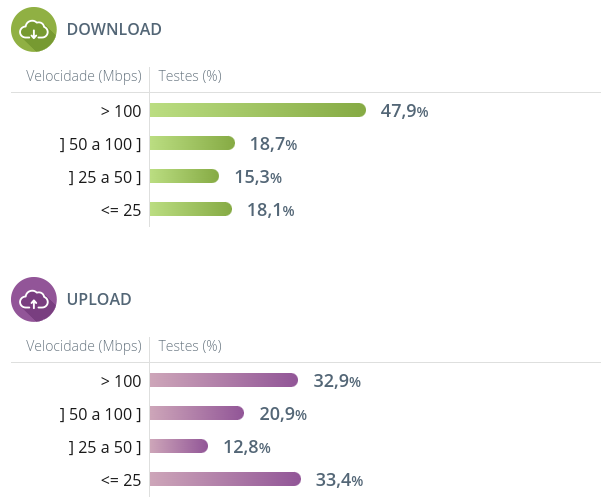
\includegraphics[width=0.5\linewidth]{figs/ch_2_netmed.png}
    \caption{Internet speed distribuition in Portugal\cite{ANACOM2023EstastisticasNET.mede}}
    \label{fig:ch_2_netmed.png}
\end{figure}

\subsubsection{Channel Estimation}
\par In wireless communications systems, the transmitted signals will be affected by various channel impairments. To efficiently decode received signals in \ac{mimo} systems, receivers must have knowledge of the channel through which the data have been propagated. This is usually done by channel estimation techniques.

\par For Pilot-Based Channel Estimation, the transmitter will send known signals, pilots, along with the data that is being transmitted. The receiver will then compare the signals it receives with what was expected for the signal to look like. This way, it can determine the channel's characteristics. The simplicity of this approach makes it the most common approach to determine the characteristics of the channel.

\par Blind Channel Estimation, as the name implies, relies only on the information it receives, without the presence of any pilots. It then performs a statistical analysis of the signals received in order to estimate the properties of the channel. The fact that this method does not have to send any pilot means that it can become more bandwidth-efficient, but will overall be more complex and difficult to implement than pilot-based channel estimation.

\par Semi-Blind Channel Estimation is a method that combines both blind and pilot based channel estimation. This method is the most attractive for use in \ac{mumimo} and \ac{mmimo} systems. This technique relies on knowledge of past experiments (training information) for the blind part and data symbols for the pilot-based approach. This helps to reduce the contamination of the bandwidth with unnecessary pilots, while being less complex and based on pure blind channel estimation\cite{Nayebi2018Semi-blindSystems}.

\subsubsection{Interference Cancellation}
\par Interference is one of the major challenges wireless communications can face. \ac{mimo} systems can have interference arising from various sources such as co-channel interference from other users, interference from neighboring systems or antennas, etc.

\par Linear Interference Cancellation has already been explained earlier. These techniques are Zero Forcing and Minimum Mean Square Error, and as the base plate for \ac{mimo} systems to work were presented first.

\par Non-Linear Interference Cancellation techniques such as \ac{sic} and \ac{pic} can also be used.

\par The first method allows a receiver to receive two signals at the same time and still be able to distinguish them correctly. It happens when the receiver can properly decode the strongest signal, and then, by subtracting this signal to the combined one that was received, extract the weakest signal received.

\par \ac{pic} is also simple, as it attempts to remove interference from all users simultaneously instead of sequentially as \ac{sic}. It tries to estimate the interference caused by each user's signal on every other signal. It then subtracts this interference for each user, in parallel for all users. Afterwards, the data obtained is reanalyzed. If it does not make sense, the process repeats until the signals have been detected accurately\cite{Divsalar1998ImprovedCDMA}.
